%%%%%%%%%%%%%%%%%%%%%%%%%%%%%%%%%%%%%%%%%
% Beamer Presentation
% LaTeX Template
% Version 1.0 (10/11/12)
%
% This template has been downloaded from:
% http://www.LaTeXTemplates.com
%
% License:
% CC BY-NC-SA 3.0 (http://creativecommons.org/licenses/by-nc-sa/3.0/)
%
%%%%%%%%%%%%%%%%%%%%%%%%%%%%%%%%%%%%%%%%%

%----------------------------------------------------------------------------------------
%	PACKAGES AND THEMES
%----------------------------------------------------------------------------------------

\documentclass{beamer}

\mode<presentation> {

% The Beamer class comes with a number of default slide themes
% which change the colors and layouts of slides. Below this is a list
% of all the themes, uncomment each in turn to see what they look like.

%\usetheme{default}
%\usetheme{AnnArbor}
%\usetheme{Antibes}
%\usetheme{Bergen}
%\usetheme{Berkeley}
%\usetheme{Berlin}
%\usetheme{Boadilla}
%\usetheme{CambridgeUS}
%\usetheme{Copenhagen}
%\usetheme{Darmstadt}
%\usetheme{Dresden}
%\usetheme{Frankfurt}
%\usetheme{Goettingen}
%\usetheme{Hannover}
%\usetheme{Ilmenau}
%\usetheme{JuanLesPins}
%\usetheme{Luebeck}
\usetheme{Madrid}
%\usetheme{Malmoe}
%\usetheme{Marburg}
%\usetheme{Montpellier}
%\usetheme{PaloAlto}
%\usetheme{Pittsburgh}
%\usetheme{Rochester}
%\usetheme{Singapore}
%\usetheme{Szeged}
%\usetheme{Warsaw}

% As well as themes, the Beamer class has a number of color themes
% for any slide theme. Uncomment each of these in turn to see how it
% changes the colors of your current slide theme.

%\usecolortheme{albatross}
%\usecolortheme{beaver}
%\usecolortheme{beetle}
%\usecolortheme{crane}
%\usecolortheme{dolphin}
%\usecolortheme{dove}
%\usecolortheme{fly}
%\usecolortheme{lily}
%\usecolortheme{orchid}
%\usecolortheme{rose}
%\usecolortheme{seagull}
%\usecolortheme{seahorse}
%\usecolortheme{whale}
%\usecolortheme{wolverine}

%\setbeamertemplate{footline} % To remove the footer line in all slides uncomment this line
%\setbeamertemplate{footline}[page number] % To replace the footer line in all slides with a simple slide count uncomment this line

%\setbeamertemplate{navigation symbols}{} % To remove the navigation symbols from the bottom of all slides uncomment this line
}

\usepackage{graphicx} % Allows including images
\usepackage{booktabs} % Allows the use of \toprule, \midrule and \bottomrule in tables
\usepackage{wrapfig}
\usepackage{hyperref}
%----------------------------------------------------------------------------------------
%	TITLE PAGE
%----------------------------------------------------------------------------------------

\title[BumpGo]{Nocom-Pila BumpGo} % The short title appears at the bottom of every slide, the full title is only on the title page

\author{Nocom-Pila} % Your name

\institute[URJC] % Your institution as it will appear on the bottom of every slide, may be shorthand to save space
{
Universidad Rey Juan Carlos  \\ % Your institution for the title page
\medskip
\textit{nocompila@gmail.com} % Your email address
}
\date{\today} % Date, can be changed to a custom date

\begin{document}



%----------------------------------------------------------------------------------------
%	PRESENTATION SLIDES
%----------------------------------------------------------------------------------------

%------------------------------------------------
%---------------------------
\begin{frame}
\titlepage % Portada.
\end{frame}
%------------------------------------ Primera diapo.
\begin{frame}

\frametitle{BumpGo} % Table of contents slide, comment this block out to remove it
\framesubtitle{State machine}

\centering
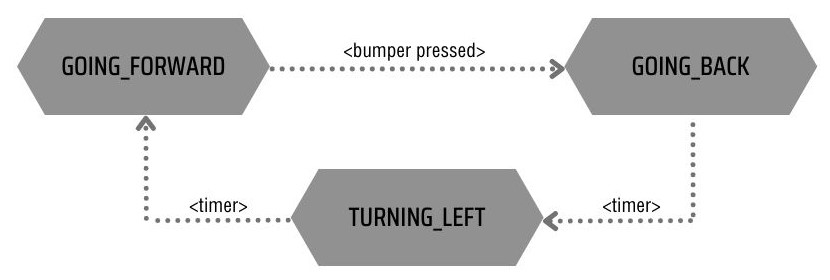
\includegraphics[height=3cm]{Bumpgobasic.jpeg}

\begin{itemize}
	\item Go forward. \\ \item Bumper.\\ \item Stop.
	\item Go backward. \\ \item Stop.\\ \item Turn left.\\ \item Go forward again.
	
\end{itemize}

\end{frame}
%---------------------------------Segunda diapo.
\begin{frame}
\frametitle{BumpGo}
\framesubtitle{Implementations}
\begin{block}{Implementations}
		In case that bumper crashed, kobuki is going to go back, stop, turn left and go 			forward again.
\end{block}
\end{frame}

\begin{frame}
\frametitle{BumpGo} 
\framesubtitle{Sensor used}
\begin{block}{Bumper}
	
	This sensor measure 1 while it is crashed with object and measure 0 when it is 			    released.
	
\end{block}

\end{frame}
%----------------------------- Tercera diapo.

\begin{frame}
\frametitle{BumpGo advanced}
\framesubtitle{State machine}	

\centering
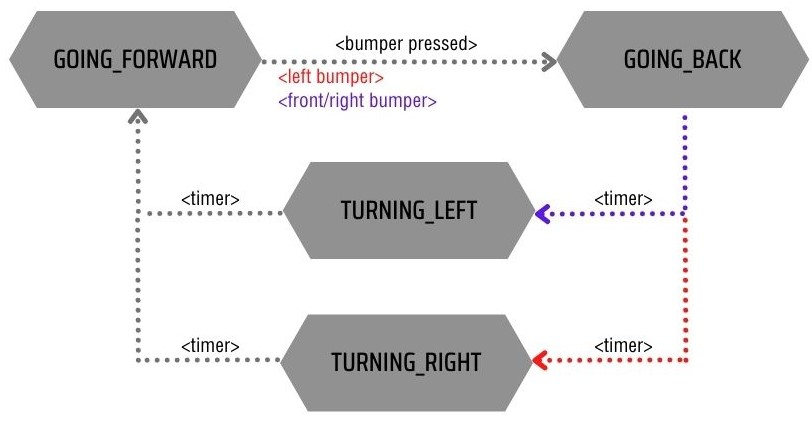
\includegraphics[height=3cm]{Bumpgoadvanced.jpg}

\begin{itemize}

	\item Go forward. \\ \item Bumper.\\ \item Stop.
	\item Go backward. \\ \item Stop.\\ \item Turn left or right.\\ \item Go forward again.
\end{itemize}
\end{frame}


%----------------
\begin{frame}
\frametitle{BumpGo advanced}
\framesubtitle{Implementations}
\begin{block}{Turning sense}
	We added 2 turning sense. This is,in case right bumper crash, kobuki have to turn to
	left sense, and vice versa.
\end{block}
\begin{block}{Leds}
	We implemented led1 and led2 to this BumpGo version. While kobuki is turning to the left sense, led1 is shining. Same with right sense with the led2.
\end{block}
\end{frame}
%---------------------------- Cuarta diapo.


\begin{frame}
\frametitle{BumpGo advanced}
\framesubtitle{Sensor used}

\begin{block}{Bumper}
	
	This sensor measure 1 while it is crashed with object and measure 0 when it is 			    released.
	
\end{block}

\end{frame}


%-------------------------------------------- Quinta diapo.

\begin{frame}
\frametitle{BumpGo Laser}
\framesubtitle{States machine}

\centering
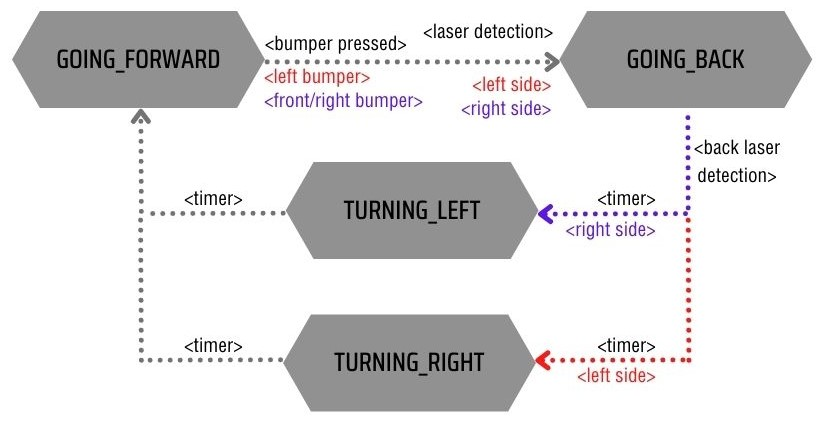
\includegraphics[height=3cm]{Bumpgolaser.jpg}

\begin{itemize}

	\item Go forward. \\ \item Rplidar or bumper.\\ \item Stop.
	\item Go backward while kobuki can. \\ \item Stop.\\ \item Turn left or right.\\ \item Go forward again.

\end{itemize}



\end{frame}

%-----------------------------------------------Sexta diapo
\begin{frame}
\frametitle{BumpGo Laser}
\framesubtitle{Implementations}
\begin{block}{Turning Sense}
	We added 2 turning sense. So, in case that rplidar measure a distance lower than our min distance setted, and its come from left side sweep, kobuki have to turns to
	right sense, and vice versa. In case, that measurement comes from forward kobuki turn to left sense by default.
\end{block}

\begin{block}{Leds}
	We implemented led1 and led2 to this BumpGo version. While kobuki is turning to the left sense, led1 is shining. Same with right sense with the led2.
\end{block}


\end{frame}
%------------------------------Septima diapo.


\begin{frame}
\frametitle{BumpGo Laser}
\framesubtitle{Implementations}

\begin{block}{Security system}
	
	In case that kobuki is going backwards to change his direction, it will  go 			backwards as long as nothing is close behind.
	In case there is something behind it, it will stop going backwards and changes to the next state.

\end{block}
\centering
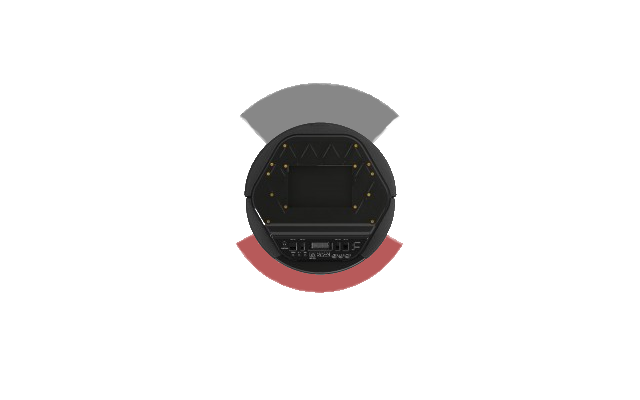
\includegraphics[width=0.5\textwidth]{angle.jpeg}

\end{frame}


%------------------------------------------------Octava diapo.
\begin{frame}
\frametitle{BumpGo Laser}
\framesubtitle{Implementations}

\begin{block}{Bumper}
	In case that something forward is bellow rpilidar, it is not going to be measure it. Due to this, we added bumper sensor to measure it.

\end{block}

\centering
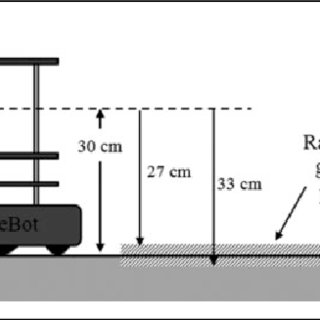
\includegraphics[width=0.35\textwidth]{levels.jpeg}



\end{frame}



%-------------------------------------------------Novena diapo.

\begin{frame}
\frametitle{BumpGo Laser}
\framesubtitle{Sensors used}

\begin{block}{Bumper}
	This sensor measure 1 while it is crashed with object and measure 0 when it is 			    released.

\end{block}

\begin{block}{Rplidar}
	
	This sensor measure 360 degrees at a range of 16 meters.
\end{block}

\end{frame}

%---------------------------------------Septima diapo.


%------------------------------------------------
\begin{frame}
\begin{itemize}
\frametitle{Contributors}
	\item Víctor Bárcena  \textit{v.barcena.2020@alumnos.urjc.es}
	\item Javier Mayorga    \textit{j.mayorga.2020@alumnos.urjc.es}
	\item Marvin Pancracio \textit{m.pancracio.2020@alumnos.urjc.es}
	\item Moisés Muñoz    \textit{m.munoz.2020@alumnos.urjc.es}
\end{itemize}
\end{frame}

\begin{frame}
\Huge{\centerline{The End}}

\centering
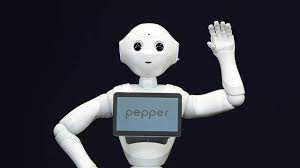
\includegraphics[width=0.5\textwidth]{p.jpeg}

\end{frame}

%----------------------------------------------------------------------------------------

\end{document} 